\subsection{Brennweitenbestimmung mit der Methode von Bessel}

Mithilfe von Gleichung \ref{eqn:brenn1} kann in diesem Fall die Brennweite über den Abstand der beiden Positionen der Linse $d$ und den Abstand zwischen Gegenstand und Schirm $e$ umformuliert werden als
\begin{equation}
  f=\frac{e^2-d^2}{4e} \text{.}
  \label{eqn:brenn2}
\end{equation}

\begin{table}
  \caption{Messwerte ohne einen Farbfilter.}
  \label{tab:bessel1}
  \centering
  \begin{tblr}{
    colspec={S[table-format=1.1] S[table-format=1.1] S[table-format=1.1] };
    row{1}={guard, mode=maths};
  }
  \toprule
  P_{L_1} \mathbin{/} \unit{\centi\meter}  & P_{L_2} \mathbin{/} \unit{\centi\meter} & P_S \mathbin{/} \unit{\centi\meter} \\
  \midrule
  38.5  &  54.6   &  70.0     \\
  37    &  60.7   &  75.0     \\
  36.6  &  66.4   &  80.0     \\
  36.1  &  71.6   &  85.0     \\
  35.9  &  76.7   &  90.0     \\
  35.8  &  82.1   &  95.0     \\
  35.8  &  87.2   &  100.0    \\
  35.4  &  92.5   &  105.0    \\
  35.2  &  97.5   &  110.0    \\
  35.2  &  102.7  &  115.0    \\  
  \bottomrule
  \end{tblr}
\end{table}

Daraus lassen sich $d$ und $e$ berechnen mit
\begin{align}
   & d=P_{L_2}-P_{L_1} \\
   & e=P_S-P_G \text{.}
\end{align}
Der errechnete Mittelwert für die Brennweite $f$ beträgt dann nach Gleichung \ref{eqn:brenn2} $\qty{9.80(0.06)}{\centi\meter}$

\begin{table}[H]
  \centering
  \label{tab:bessel2}
  \caption{Messwerte mit einem blauen Filter.}
  \begin{tblr}{
    colspec={S[table-format=1.1] S[table-format=1.1] S[table-format=1.1] };
    row{1}={guard, mode=maths};
    }
    \toprule
    P_{L_1} \mathbin{/} \unit{\centi\meter}  & P_{L_2} \mathbin{/} \unit{\centi\meter} & P_S \mathbin{/} \unit{\centi\meter} \\
    \midrule
    38.2  &  54.8  &  70.0  \\
    37.2  &  60.5  &  75.0  \\
    36.5  &  66.5  &  80.0  \\
    36.4  &  71.8  &  85.0  \\
    36.0  &  76.9  &  90.0  \\
    \bottomrule
  \end{tblr}
\end{table}


\begin{table}[H]
  \centering
  \label{tab:bessel3}
  \caption{Messwerte mit einem rotem Filter.}
  \begin{tblr}{
    colspec={S[table-format=1.1] S[table-format=1.1] S[table-format=1.1] };
    row{1}={guard, mode=maths};
    }
    \toprule
    P_{L_1} \mathbin{/} \unit{\centi\meter}  & P_{L_2} \mathbin{/} \unit{\centi\meter} & P_S \mathbin{/} \unit{\centi\meter} \\
    \midrule
    38.4  &  54.7  &  70.0 \\
    37.3  &  60.7  &  75.0 \\
    36.8  &  66.3  &  80.0 \\
    36.3  &  71.6  &  85.0 \\
    36.3  &  76.7  &  90.0 \\
    \bottomrule
  \end{tblr}
\end{table}

Nach der gleichen Methode, wie bei der Messung ohne Filter, wird die Brennweite der Linse bestimmt mit den Farbfiltern. Dabei ergeben sich Brennweiten von $f_b=\qty{9.75(0.06)}{\centi\meter}$ und $f_r=\qty{9.82(0.08)}{\centi\meter}$.

\subsection{Brennweitenbestimmung mit der Methode von Abbe}

\begin{table}[H]
  \centering
  \caption{Messdaten zur Bestimmung der Brennweite einer Linse nach der abbeschen Methode.}
  \label{tab:abbe}
  \begin{tblr}{
    colspec={S[tableformat=1.1] S[tableformat=1.1] S[tableformat=1.1]};
    rom{1}={guard, mode=maths};
    }
    \toprule
    P_L \mathbin{/} \unit{\centi\meter} & P_S \mathbin{/} \unit{\centi\meter} & B \mathbin{/} \unit{\centi\meter} \\
    \midrule
    50.0   &   120.0  &  5.5  \\
    55.0   &   114.0  &  4.0  \\
    60.0   &   112.5  &  3.2  \\
    65.0   &   112.5  &  2.5  \\
    70.0   &   114.5  &  2.2  \\
    75.0   &   118.6  &  2.0  \\
    80.0   &   122.4  &  1.8  \\
    85.0   &   125.1  &  1.7  \\
    90.0   &   128.6  &  1.2  \\
    95.0   &   133.4  &  1.0  \\  
    \bottomrule
  \end{tblr}
\end{table}


\begin{figure}
    \caption{Der Abstand zwischen dem Referenzpunkt und dem Gegenstand $g$ gegen $1+\frac{1}{V}$. (oben) \\ Der Abstand zwischen dem Schirm und dem Referenzpunkt $b$ gegen $1+V$.(unten)}
    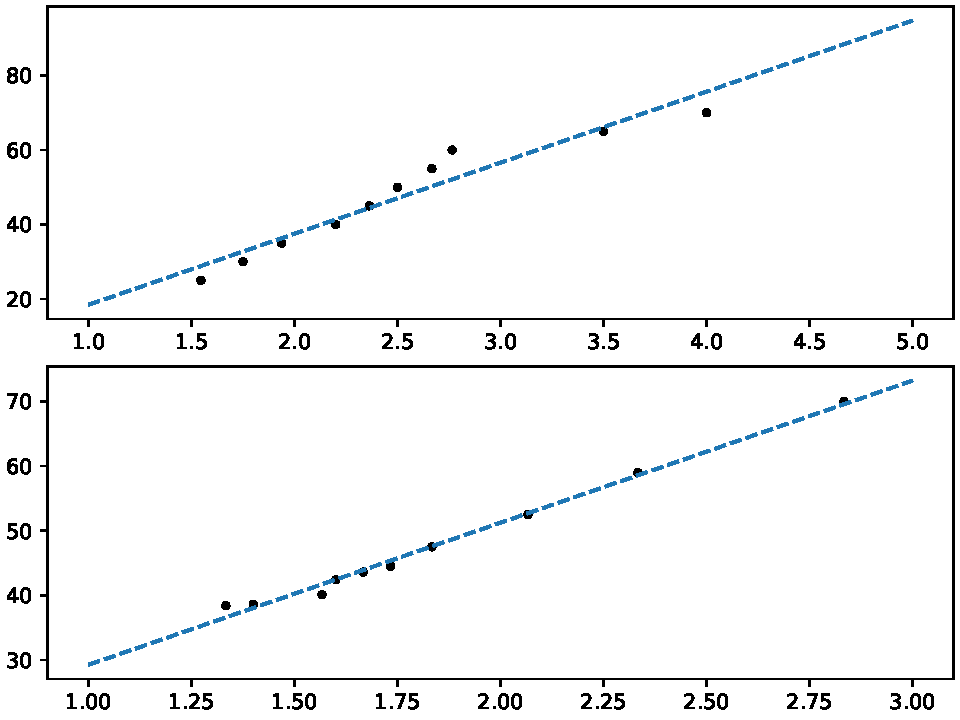
\includegraphics{abbe.pdf}
    \label{fig:abbe}
\end{figure}

Anhand der Formeln \ref{eqn:abbe} ergibt sich das die gemittelte Brennweite der kombinierten Linsen $f=\qty{20.5(1.0)}{\centi\meter}$ beträgt. Die Hauptebene $H'$ befindet sich $\qty{7.24(1.32)}{\centi\meter}$ vom Referenzpunkt
weit weg und die Ebene $H$ ist $\qty{-0.64(5.02)}{\centi\meter}$ weit weg.